\documentclass[letterpaper,11pt,onecolumn]{article}
\usepackage[utf8]{inputenc}
\usepackage{fontenc}
\usepackage{amsmath}
\usepackage{graphicx}
\usepackage{subfigure}
\usepackage{xcolor}
\usepackage[top=1.85cm, left=2cm, bottom=2cm, right=2cm]{geometry}
\setlength{\parindent}{0cm}
\usepackage{booktabs}
\usepackage{biblatex}
\addbibresource{References.bib}
%\usepackage{cite}
\usepackage{enumitem}
\usepackage{hyperref}
\usepackage{comment}
\usepackage{multicol}
\usepackage{lipsum}
\usepackage{bm}


\title{Schwartzschild Geometry: Metric, Geodesics and Black Holes}
\author{ Alejandro Gómez$^1$\thanks{\href{mailto:alejandro.cadavid@correounivalle.edu.co}{alejandro.cadavid@correounivalle.edu.co}} , Juan E. Bedoya$^1$\thanks{\href{mailto:juan.esteban.bedoya@correounivalle.edu.co}{juan.esteban.bedoya@correounivalle.edu.co}} , Nicolle Tello$^1$\thanks{\href{mailto:nicolle.tello@correounivalle.edu.co}{nicolle.tello@correounivalle.edu.co}} , Stiven Londoño$^1$\thanks{\href{mailto:danilo.londono@correounivalle.edu.co}{danilo.londono@correounivalle.edu.co}} . \\ $^1$\textit{Departamento de Física, Universidad del Valle} }
\date{\today}

\begin{document}

\maketitle

\begin{abstract}
    This document is part of the final assignment of the \textit{Introduction to Relativity} course, which focused on studying a simple but powerful result of general relativity. Here we present the Schwarzschild geometry, discuss some general aspects and show their consequences, such as the corrections to planetary motion, deflection of photons due to gravity and natural emergence of black holes. Those results serve as a motivation to study more advanced topics and dive into cosmology. 
    
\end{abstract}

\tableofcontents

\newpage


\section{Introduction}\label{intro}

In 1916 Albert Einstein published \emph{Relativity: The Special and General Theory} \cite{einstein_uber_2009}, originally written in German and translated four years later into English by Robert W. Lawson. This book introduced a new theory of space-time, in which time was no longer an absolute quantity and several paradoxes appeared. Nevertheless, it was proved right by several experiments carried out years later \cite{hobson_efstathiou_lasenby_2006}. Einstein's book was divided into two parts, the first concerning to the special relativity, which was built on the flat Minkowski space, while the second part provided a theory of gravitation, which is the one of interest in this document. 

The general theory explained gravity from a geometrical approach instead of being an interaction as in Newtonian mechanics. One of the most important results of this theory was the so-called Einstein field equations. Let $G_{\mu \nu}$, $ g_{\mu \nu}$, $\Lambda$, $\kappa$ and $T_{\mu \nu}$ be the Einstein tensor, metric tensor, cosmological constant, gravitational constant and Energy-momentum tensor, respectively, then the following holds

\begin{equation} \label{field}
    G_{\mu \nu} + \Lambda g_{\mu \nu} = \kappa T_{\mu \nu} 
\end{equation}

where the LHS accounts for the geometry of the space time whereas the RHS is the matter content of the space. Therefore, matter curves the space-time, modifying the geodesics, which are the paths followed by particles due to the least-action principle. 

On the other hand, in 1916 Karl Schwarzschild found a solution of \ref{field} outside a spherical neutral and non-spinning mass \cite{1916SPAW.......189S}. The solution is shown in form of a metric that depends on several parameters that will be discussed in the next sections. The Schwarzschild metric explained how photons trajectories are affected by gravity even though they are massless. It also gave relativistic corrections to planetary motion in the form of elliptical precession and finally, introduced some properties of Black Holes. Thus, this theory contains a lot of interesting physical phenomena which will be discussed throughout this document. 

Finally, this document is based on \cite{hobson_efstathiou_lasenby_2006}, so the interested reader can refer to it for more details and problem sets. 

\section{Metric}\label{metric}

\subsection{The general static isotropic metric}

To construct the metric for a spherically symmetric gravitational field, generated by a massive spherical object, one should start with the general expression for the line element, as shown:

\begin{equation}
d s^{2}=g_{\mu \nu} d x^{\mu} d x^{\nu}\label{lineelement}
\end{equation}

Since it is needed a static isotropic metric, for an easy approach one should start constructing just a spatially isotropic metric, which is more general. For this, one seeks after a line element that depends only on rotational invariants of the spacelike coordinates of $x^i$ and their differentials, such as

\begin{equation}
\vec{x} \cdot \vec{x}, \quad d \vec{x} \cdot d \vec{x}, \quad \vec{x} \cdot d \vec{x}\nonumber
\end{equation}

it is usually noted that $x^i=(x^0,x^1,x^2,x^3)=(t,\vec{x})$. Then, following its most general form, the spatially isotropic metric is:

\begin{equation}
d s^{2}=A(t, r) d t^{2}-B(t, r) d t \vec{x} \cdot d \vec{x}-C(t, r)(\vec{x} \cdot d \vec{x})^{2}-D(t, r) d \vec{x}^{2}
\label{genmetric}
\end{equation}

using $A$, $B$, $C$ and $D$ as arbitrary functions of $t$ and $r$. Using the usual spherical polar coordinates, one gets:

\begin{equation}
\vec{x} \cdot \vec{x}=r^{2}, \quad \vec{x} \cdot d \vec{x}=r d r, \quad d \vec{x} \cdot d \vec{x}=d r^{2}+r^{2} d \theta^{2}+r^{2} \sin ^{2} \theta d \phi^{2} \nonumber
\end{equation}

so the metric from Eq. \ref{genmetric} takes the form,

\begin{equation}
\begin{aligned}
d s^{2}=& A(t, r) d t^{2}-B(t, r) r d t d r-C(t, r) r^{2} d r^{2} \\
&-D(t, r)\left(d r^{2}+r^{2} d \theta^{2}+r^{2} \sin ^{2} \theta d \phi^{2}\right)
\end{aligned}\nonumber
\end{equation}

which can be rewritten as 

\begin{equation}
d s^{2}=A(t, r) d t^{2}-B(t, r) d t d r-C(t, r) d r^{2}-D(t, r)\left(d \theta^{2}+\sin ^{2} \theta d \phi^{2}\right)
\label{genmet2}
\end{equation}
by absorbing some terms to the arbitrary functions. One can also define a new radial and a timelike coordinate, such as 
\begin{equation}
\bar{r}^{2}=D(t, r) \quad \text{and} \quad d \bar{t}=\Phi(t, \bar{r})\left[A(t, \bar{r}) d t-\frac{1}{2} B(t, \bar{r}) d \bar{r}\right]\nonumber
\end{equation}
from the second one we find that 
\begin{equation}
A d t^{2}-B d t d \bar{r}=\frac{1}{A \Phi^{2}} d \bar{t}^{2}-\frac{B}{4 A} d \bar{r}^{2} \nonumber
\end{equation}
that allows to define new arbitrary functions $\bar{A}=1 /\left(A \Phi^{2}\right)$ and $\bar{B}=C+B /(4 A)$. So Eq. \ref{genmet2} can be written as:
\begin{equation}
d s^{2}=A(t, r) d t^{2}-B(t, r) d r^{2}-r^{2}\left(d \theta^{2}+\sin ^{2} \theta d \phi^{2}\right)\nonumber
\end{equation}
by removing all the bars over the new variables.\\
With that, the spatially isotropic metric is found. To find the static isotropic metric, one just needs to write the metric as independent of the timelike coordinate, this means: 
\begin{equation}
d s^{2}=A( r) d t^{2}-B( r) d r^{2}-r^{2}\left(d \theta^{2}+\sin ^{2} \theta d \phi^{2}\right)\nonumber
\end{equation}
Thus one gets the static isotropic metric, but it's still needed to solve the empty-space field equations
%------------------------------------------------------------------------------------
\subsection{Solution to the empty-space field equations}
To solve the empty-space field equations, we must have a Ricci tensor that vanishes. This is:
\begin{equation}
        R_{\mu \nu}=\partial_{\nu} \Gamma_{\mu \sigma}^{\sigma}-\partial_{\sigma} \Gamma_{\mu \nu}^{\sigma}+\Gamma_{\mu \sigma}^{\rho} \Gamma_{\rho \nu}^{\sigma}-\Gamma_{\mu \nu}^{\rho} \Gamma_{\rho \sigma}^{\sigma}=0
        \label{ricci}
\end{equation}

having in mind that
\begin{equation}
\Gamma_{\mu \nu}^{\sigma}=\frac{1}{2} g^{\sigma \rho}\left(\partial_{\nu} g_{\rho \mu}+\partial_{\mu} g_{\rho \nu}-\partial_{\rho} g_{\mu \nu}\right)
\label{conn}
\end{equation}

To solve this, we start with the non-zero elements of the metric, $g_{\mu\nu}$
  $$
\begin{array}{ll}
g_{00}=A(r), & g^{00}=1 / A(r) \\
g_{11}=-B(r), & g^{11}=-1 / B(r) \\
g_{22}=-r^{2}, & g^{22}=-1 / r^{2} \\
g_{33}=-r^{2} \sin ^{2} \theta, & g^{33}=-1 /\left(r^{2} \sin ^{2} \theta\right)
\end{array}
$$
With these components of the metric one can find the connection coefficients, by replacing them in Eq. \ref{conn}. The non-zero coefficients found are: 
$$
\begin{array}{lll}
\Gamma_{01}^{0}=A^{\prime} /(2 A), & \Gamma_{00}^{1}=A^{\prime} /(2 B), & \Gamma_{11}^{1}=B^{\prime} /(2 B) \\
\Gamma_{22}^{1}=-r / B, & \Gamma_{33}^{1}=-\left(r \sin ^{2} \theta\right) / B, & \Gamma_{12}^{2}=1 / r \\
\Gamma_{33}^{2}=-\sin \theta \cos \theta, & \Gamma_{13}^{3}=1 / r, & \Gamma_{23}^{3}=\cot \theta
\end{array}
$$
By placing these into Eq. \ref{ricci}, one can find that only the diagonal of the Ricci tensor is non-zero, as follows:
\begin{eqnarray}
\centering
R_{00}&=&-\frac{A^{\prime \prime}}{2 B}+\frac{A^{\prime}}{4 B}\left(\frac{A^{\prime}}{A}+\frac{B^{\prime}}{B}\right)-\frac{A^{\prime}}{r B} \label{r00}\\
R_{11}&=&\frac{A^{\prime \prime}}{2 A}-\frac{A^{\prime}}{4 A}\left(\frac{A^{\prime}}{A}+\frac{B^{\prime}}{B}\right)-\frac{B^{\prime}}{r B} \label{r11}\\
R_{22}&=&\frac{1}{B}-1+\frac{r}{2 B}\left(\frac{A^{\prime}}{A}-\frac{B^{\prime}}{B}\right)\label{r22} \\
R_{33}&=&R_{22} \sin ^{2} \theta\label{r33}
\end{eqnarray}
 Since it's needed that every component of this tensor to be equal to zero, one can obtain the relation
 \begin{equation}
     A'B+AB'=0\nonumber
 \end{equation}
 by adding B/A times Eq. \ref{r00} to Eq. \ref{r11}. This leads to $AB=\alpha=constant$, from which we can substitute $B$ into \ref{r22} and get a relation of just $A$ and $A'$ as $A+rA'=\alpha$. This can also be written as
 \begin{equation}
\frac{d(r A)}{d r}=\alpha, \nonumber
\end{equation}
so that when integrating one can get expressions for both arbitrary constants,
\begin{equation}
A(r)=\alpha\left(1+\frac{k}{r}\right) \quad \text { and } \quad B(r)=\left(1+\frac{k}{r}\right)^{-1} \nonumber
\end{equation}
One can find the value of $\alpha$ and $k$ by considering the weak-field limit, getting that $k=-2 G M / c^{2}$ and $\alpha=c^{2}$. With all of this, the Schwarzschild metric for the empty spacetime outside a spherical body of mass M takes the form of: 
\begin{equation}
d s^{2}=c^{2}\left(1-\frac{2 G M}{c^{2} r}\right) d t^{2}-\left(1-\frac{2 G M}{c^{2} r}\right)^{-1} d r^{2}-r^{2} d \theta^{2}-r^{2} \sin ^{2} \theta d \phi^{2}\nonumber
\end{equation}
which can be simplified by using $\mu=GM/c^2$
\begin{equation}
d s^{2}=\underbrace{c^{2}\left(1-\frac{2 \mu}{r}\right)}_{g_{00}} d t^{2} \underbrace{-\left(1-\frac{2 \mu}{r}\right)^{-1}}_{g_{11}} d r^{2}\underbrace{-r^{2}}_{g_{22}} d \theta^{2}\underbrace{-r^{2} \sin ^{2}\theta}_{g_{33}}  d \phi^{2}
\label{metric}
\end{equation}
This is the expression that will constantly be used from this point onwards.

\section{Geodesics}


The geodesics are, by definition, the length-minimizing curves of the geometry. These curves are expected to be followed by the particles moving around some gravitational field curving the spacetime. Then, we can find the trajectories of massive and massless particles (photons) from the geodesic equations. If these curves are affinely parametrized, say by $\sigma$, they satisfy the following set of equations

\begin{equation}
    \frac{d^2 x^\mu}{d\sigma^2} + \Gamma^{\mu}_{\nu \rho} \frac{dx^\nu}{d\sigma} \frac{dx^\rho}{d\sigma} = 0
\end{equation}

In the same fashion, we can define a Lagrangian $\mathcal{L} = g_{\mu \nu}  \dot{x}^\mu \dot{x}^\nu$ and find the set of action-minimizing (Euler-Lagrange) equations

\begin{equation}\label{Euler-Lagrange}
\frac{d}{d\sigma} \left( \frac{\partial \mathcal{L}}{\partial \dot{x}^\mu}\right) - \frac{\partial \mathcal{L}}{\partial x^\mu} = 0
\end{equation}

which are equivalent to the geodesic equations. We will use the Lagrangian approach as it resembles basic Classical Mechanics and is easier to use. 

Using Eq. {\color{red} REF}, the Lagrangian is given by 

\begin{equation} \label{Lagrangian}
    \mathcal{L} = c^{2}\left( 1-\frac{2\mu}{r} \right)\dot{t}^{2}-\left( 1-\frac{2\mu}{r}\right)^{-1}\dot{r}^{2}-r^{2}\left(\dot{\theta}^{2}+sen^{2}\theta\right)\dot{\phi}^{2}
\end{equation}

From Eq. \ref{Euler-Lagrange}, it follows that

\begin{itemize}
    \item $x^0 = ct$
    $$\frac{d}{d\sigma} \left( \frac{\partial \mathcal{L}}{\partial \dot{t}}\right) - \frac{\partial \mathcal{L}}{\partial t} = 0$$  $$\left( 1 - \frac{2 \mu}{r} \right) \dot{t} = k$$
    
    \item $x^1 = r$
    $$\frac{d}{d\sigma} \left( \frac{\partial \mathcal{L}}{\partial \dot{r}}\right) - \frac{\partial \mathcal{L}}{\partial r} = 0 $$
    $$\left( 1 - \frac{2 \mu}{r} \right)^{-1} \ddot{r} + \frac{2\mu}{r^2} \dot{t}^2 - \left( 1 - \frac{2 \mu}{r} \right)^{-2} \frac{\mu}{r^2} \dot{r}^2 - r \left( \dot{\theta}^2 + \sin^2 \theta \dot{\phi}^2  \right) = 0$$
    
    \item $x^2 = \theta$
    $$\frac{d}{d\sigma} \left( \frac{\partial \mathcal{L}}{\partial \dot{\theta}}\right) - \frac{\partial \mathcal{L}}{\partial \theta} = 0 $$
    $$\ddot{\theta} + \frac{2}{r} \dot{r} \dot{\theta} - \sin \theta \cos \theta \dot{\phi}^2 = 0$$
    
    \item $x^3 = \phi$
     $$ \frac{d}{d\sigma} \left( \frac{\partial \mathcal{L}}{\partial \dot{\phi}}\right) - \frac{\partial \mathcal{L}}{\partial \phi} = 0 $$
     $$r^2 \sin^2 \theta \dot{\phi = h }$$
    
\end{itemize}

where $k$ and $h$ are constants of motion as both $t$ and $\phi$ are cyclic coordinates. When a variable is cyclic, its conjugated momentum is conserved. Therefore, $h$ is the angular momentum and  $k$ is related to the energy of the orbit as follows

\begin{equation}
    k = \frac{E}{m_0 c^2}
\end{equation}

where $m_0$ is the test mass. On the other hand, we can take advantage of the spherical symmetry of the metric and focus our attention to the equator. $\theta = \pi / 2$ clearly satisfies the $\theta$-equation derived above. So, our set of differential equations reduces to 

    \begin{eqnarray}
        \left( 1 - \frac{2 \mu}{r} \right) \dot{t} = k \label{t-equation} \\
        \left( 1 - \frac{2 \mu}{r} \right)^{-1} \ddot{r} + \frac{2\mu}{r^2} \dot{t}^2 - \left( 1 - \frac{2 \mu}{r} \right)^{-2} \frac{\mu}{r^2} \dot{r}^2 - r\dot{\phi}^2  = 0 \label{r-equation} \\
        r^2 \dot{\phi} = h \label{phi-equation}
    \end{eqnarray}

The motion of any particle is in principle, governed by this set of equations. For some choice of parameters, they can be solved numerically and plotted even outside the equator (See Fig. \ref{fig:general_orbit})

\begin{figure}[h!]
    \centering
    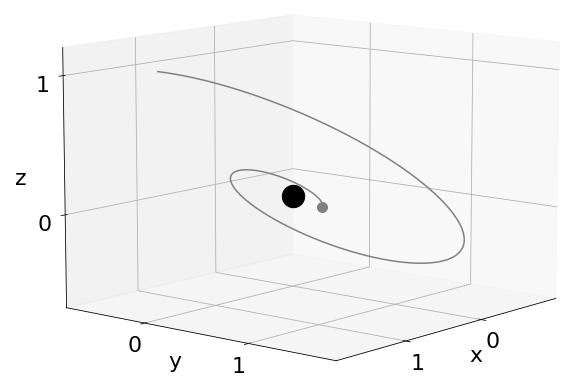
\includegraphics[width=0.6\linewidth]{Presentations/Images/2_gen_obit1.png}
    \caption{Numerical solution of the general form of the Euler-Lagrange equations. In this case, $\theta$ is arbitrary and the time coordinate is not relevant.}
    \label{fig:general_orbit}
\end{figure}

Even though the general problem could be solved, there is still much physics to be explored. For the sake of simplicity, Eq. \ref{r-equation} is replaced by the first integral $g_{\mu \nu} \dot{x^\mu} \dot{x^\nu}$. The problem is not only simplified by introducing the first integral, but also split into two branches, orbits of massive particles and massless particles, which will be discussed in the next sections.

\subsection{Massive particles}

Choosing the proper time $\tau$ as the affine parameter 

\begin{equation*}
    g_{\mu \nu} \dot{x^\mu} \dot{x^\nu} = c^2
\end{equation*}

Using Eq. {\color{red} REF} 

\begin{equation} \label{massive-r-eq}
    c^2 \left( 1 - \frac{2 \mu}{r} \right) \dot{t}^2  - \left( 1 - \frac{2 \mu}{r} \right)^{-1} \dot{r}^2 - r\dot{\phi}^2  = c^2
\end{equation}

which replaces Eq. \ref{r-equation}. These new set of equations can be solved numerically (See Fig. \ref{fig:massive-set})


\begin{figure}[h!]
    \centering
    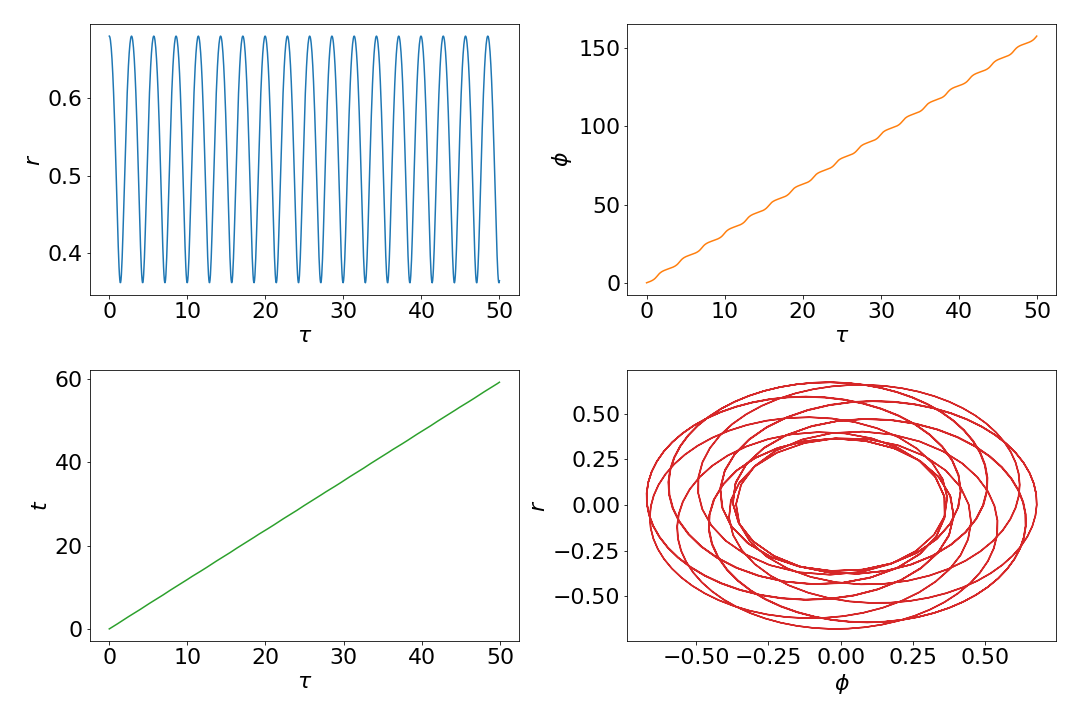
\includegraphics[width=0.8\linewidth]{Presentations/Images/2_first_orbits.png}
    \caption{Numerical solution of the Euler-Lagrange equations for massive particles at the equator, including the first integral. Notice how the trajectories are no longer ellipses as in Newtonian Mechanics. }
    \label{fig:massive-set}
\end{figure}


Inserting Eqs. \ref{t-equation} and \ref{phi-equation} into Eq. \ref{massive-r-eq} leads us to 

\begin{equation} \label{massive-r-tau}
    \dot{r}^2 + \frac{h^2}{r^2} \left( 1 - \frac{2\mu}{r}\right) - \frac{2\mu c^2}{r} = c^2 (k^2 - 1)
\end{equation}

Furthermore, we can determine $r$ as a function of $\phi$, i.e. find a direct differential equation for the trajectories. Starting from the chain rule 

\begin{equation*}
    \dot{r} = \frac{dr}{d\phi} \frac{d\phi}{d\tau} = \frac{h}{r^2} \frac{dr}{d\phi} 
\end{equation*}

and introducing the inverse of radius as a new variable 

\begin{equation*}
    u = \frac{1}{r} \longrightarrow \frac{du}{d\phi} = - \frac{1}{r^2} \frac{dr}{d\phi}
\end{equation*}

Eq. \ref{massive-r-tau} becomes

\begin{equation}
    \left( \frac{du}{d\phi} \right)^2 + u^2 = \frac{c^2}{h^2} (k^2 - 1) + \frac{2\mu c^2}{h^2} u + 2 \mu u^3
\end{equation}

After differentiating with respect to $\phi$, 

\begin{equation} \label{massive-u-eq}
    \frac{d^2u}{d \phi^2} + u = \frac{GM}{h^2} + \frac{3GM}{c^2} u^2
\end{equation}

Notice that the first term of the RHS is the classical term for the orbits, whereas the second term is the relativistic correction, which vanishes when $c\to\infty$. This allows us to start analyzing our results in terms of relativistic corrections. 

\subsubsection{Stability of orbits}

In the Newtonian case, the equation of motion is 

\begin{equation} \label{massive-traj-newton}
    \frac12 \left( \frac{dr}{dt} \right)^2  \underbrace{-\frac{GM}{r} + \frac{h^2}{2r^2}}_{V_{eff}(r)} = E
\end{equation}

In the relativistic case, it is given by Eq. \ref{massive-r-tau}

\begin{equation} \label{massive-traj-rela}
    \frac12 \left( \frac{dr}{d\tau} \right)^2  \underbrace{-\frac{\mu c^2}{r} + \frac{h^2}{2r^2} - \frac{\mu h^2}{r^3}}_{V_{eff}(r)} = \frac12 c^2 (k^2-1)
\end{equation}

The effective potential (See Fig. \ref{fig:massive-eff-V}) has some stable point depending on the angular momentum $h$. The critical points of $V_{eff}$ are 

\begin{equation}
    \left. \frac{dV_{eff}}{dr} \right|_{r=r^*} \longrightarrow r^* = \frac{h}{2\mu c^2} \left( h \pm \sqrt{h^2 - 12 \mu^2 c^2} \right)
\end{equation}

If $h^2 = 12 \mu^2 c^2$ there exists only one critical point, therefore only one circular (unstable) orbit.

\begin{figure}[h!]
    \centering
    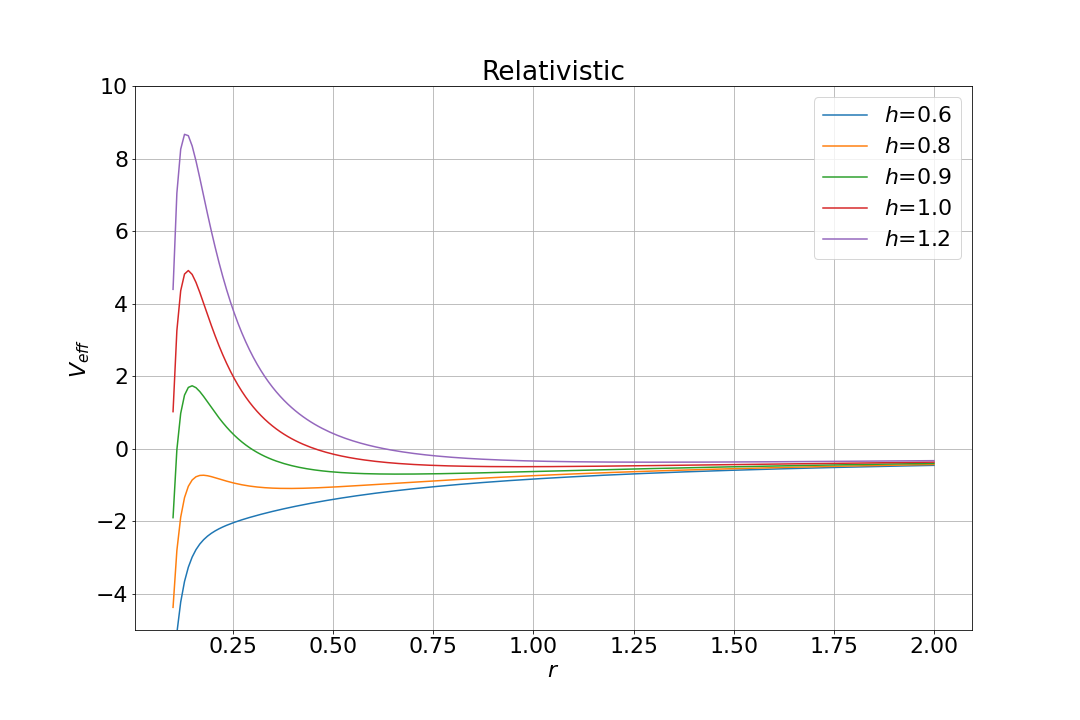
\includegraphics[width=0.75\textwidth]{Presentations/Images/2_veff_relat.png}
    \caption{Effective relativistic potential as a function of the radius for several values of angular momentum. There exists an angular momentum threshold at $h=2\sqrt{3} \mu c$ for the potential to have stable closed orbits. For example, there exists no critical point for $h=0.6$.}
    \label{fig:massive-eff-V}
\end{figure}
  

We conclude that, the minimum stable orbit satisfies $r=6\mu$. If $r < 6\mu$ the scenario is the one of Fig. \ref{fig:general_orbit}.

In the same fashion, we can compare the trajectories described by Eq. \ref{massive-traj-newton} with the ones of Eq. \ref{massive-traj-rela} and obtain Fig. \ref{fig:relnew}


\begin{figure}[h!]
    \centering
    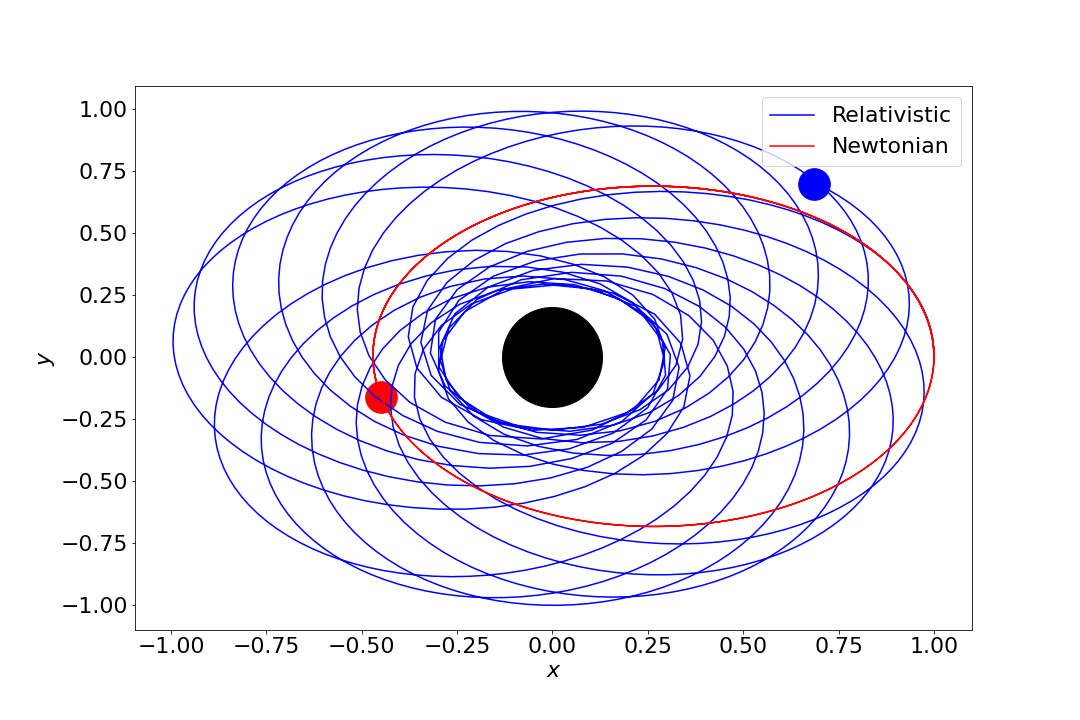
\includegraphics[width=0.8\linewidth]{Presentations/Images/2_class_rel_orbit.png}
    \caption{Numerical solution of the Newtonian and Relativistic orbits. The relativistic correction term of order $1/r^{3}$ leads to a precession of the orbit, so that the ellipses do not close but stat to shift.}
    \label{fig:relnew}
\end{figure}


Finally, we can analyze two particular cases: circular orbits and radial motion, i.e. free fall. 

\subsubsection{Radial motion: free fall}

If a test mass is falling radially, it has no angular momentum ($h=0$). So, Eq. \ref{massive-r-tau} becomes 

\begin{equation} \label{massive-radialcase-main}
    \dot{r}^2 = c^2(k^2-1) + \frac{2GM}{r}
\end{equation}

After differentiation, 

\begin{equation*}
    \ddot{r} = - \frac{GM}{r}
\end{equation*}

which has the same form of Newtonian gravity. However, it does not mean they are exactly the same, the key difference is the physical interpretation of $r$

\begin{table}[h!]
    \centering
    \begin{tabular}{l|l}
         Newtonian & Relativistic  \\ \hline
         $r$ is the radial distance and $t$ & $r$ is the distance through the metric \\
         is the universal time. & and $\tau$ is the proper time. 
    \end{tabular}
\end{table}


From Eq. \ref{massive-radialcase-main}, if the particle is released from rest, 

\begin{equation*}
    k^2 = 1 - \frac{2GM}{c^2 R}
\end{equation*}

So, for large initial distances, $k \approx 1$ and Eq. \ref{massive-radialcase-main} transforms into 

\begin{equation} \label{massive-radialcase-integrate}
    \frac{dr}{d\tau} = - \sqrt{\frac{2\mu c^2}{r}}
\end{equation}

where the negative sign accounts for the free fall, i.e. the distance decreases over time. Next, we integrate Eq. \ref{massive-radialcase-integrate} and find $r$ as a function of $\tau$, but a more interesting case is finding $r$ as a function of $t$. Using Eq. \ref{t-equation}

\begin{equation} \label{massive-radialcase-integrate-time}
    \frac{dr}{dt} = \frac{dr}{d\tau} \frac{d\tau}{dt} = - \sqrt{2\mu c^2} r^{-3/2} (r - 2\mu)
\end{equation}

The analytical solutions to Eqs. \ref{massive-radialcase-integrate} and \ref{massive-radialcase-integrate-time} are shown in Eqs. \ref{massive_ff1} and \ref{massive_ff2}, respectively. Besides, their functional behaviour is plotted in Fig. \ref{fig:massive-ff}

\begin{equation} \label{massive_ff1}
    \tau - \tau_0 = \frac23 \sqrt{\frac{r_0^3}{2\mu c^2}} -  \frac23 \sqrt{\frac{r^3}{2\mu c^2}} \label{28}
\end{equation}

\begin{equation} \label{massive_ff2}
    t - t_0 = \frac23 \left( \sqrt{\frac{r_0^3}{2\mu c^2}} - \sqrt{\frac{r^3}{2\mu c^2}} \right) + \frac{4 \mu}{c}  \left( \sqrt{\frac{r_0}{2\mu}} - \sqrt{\frac{r}{2\mu}} \right) + \frac{2\mu}{c} \log \left| \left( \frac{\sqrt{r/2\mu} + 1}{\sqrt{r/2\mu} - 1} \right) \left( \frac{\sqrt{r_0/2\mu} - 1}{\sqrt{r_0/2\mu} + 1} \right)  \right| \label{29}
\end{equation}


\begin{figure}[h!]
    \centering
    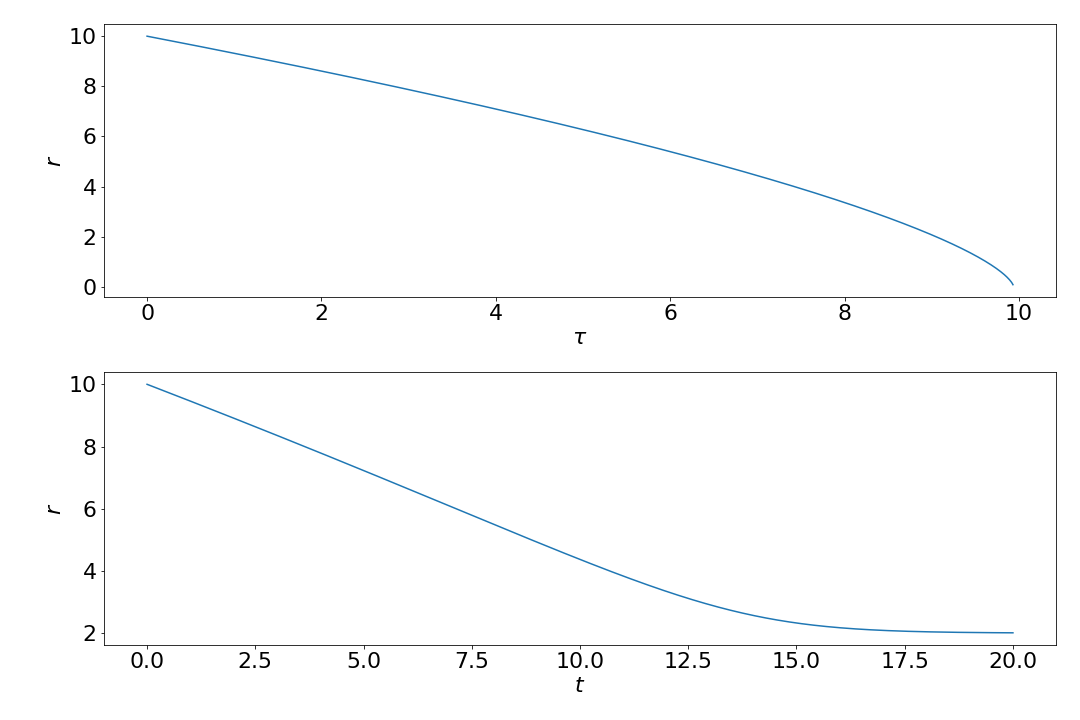
\includegraphics[width=0.8\linewidth]{Report/Images/2_radial_motion.png}
    \caption{It takes finite proper time for the particle to reach $r=0$ whereas it takes infinite universal time for it to reach $r = 2\mu$.}
    \label{fig:massive-ff}
\end{figure}


\subsubsection{Circular motion}


In this case, $\dot{r} = 0$, so Eq. \ref{massive-u-eq} becomes

\begin{equation}
    u = \frac{\mu c^2}{h^2} + 2 \mu u^2 \quad \longrightarrow \quad h = \sqrt{\frac{\mu c^2 r^2}{r-3 \mu}} 
\end{equation}
 
On the other hand, from Eq. \ref{massive-r-tau}

\begin{equation}
    k = \frac{1-2\mu/r}{\sqrt{1-3\mu/r}}
\end{equation}
 
 from these two expressions, it is clear that there exists no circular orbit at $r<3\mu$ which is consistent with the analysis made in previous sections. 
 
\subsection{Massless particles}
In the same way that the particles whit mass, for the motion of photons, the lagrange equations that were previously stated are used, these are the equations \textbf{(citar las ecuaciones aquí)}, where the interpretations of the constants is invariant. On the other hand, unlike massive particles for the photons the radial equations is replaced for by a first integral of itself of the form:
\begin{equation*}
      g_{\mu \nu}\dot{x}^{\mu}\dot{x}^{\nu}&=&0
\end{equation*}
This expression differs from the proposal in the previous case because the affine parameter is not the proper time, in this case a parameter $(\sigma)$ such that it fulfills the characteristic $p^{\mu}=\dot{x}^{\mu}$ is used.\\
Once the first integral is replaced in the equanions of motión \textbf{(citar las ecuaciones aquí)} , it follows that:
\begin{eqnarray}
      \Big(1-\frac{2\mu}{r} \Big)\dot{t}&=&k \label{f0}\\
      c^{2}\Big( 1- \frac{2\mu}{r}\Big) \dot{t}^{2}-\Big( 1- \frac{2\mu}{r}\Big)^{-1} \dot{r}^{2}-r^{2}\dot{\phi}^{2}&=&0\label{f1} \\
       r^{2}\dot{\phi}&=&h\label{f2}
\end{eqnarray}\\
To solve this system of equations, equations \ref{f0} and \ref{f2} are taken and replaced in the equation \ref{f1} arriving at:
\begin{eqnarray*}
      c^{2}\Big( 1- \frac{2\mu}{r}\Big) \dot{t}^{2}-\Big( 1- \frac{2\mu}{r}\Big)^{-1} \dot{r}^{2}-r^{2}\dot{\phi}^{2}&=&0\\
      c^{2}\overbrace{\Big( 1- \frac{2\mu}{r}\Big)^{2} \dot{t}^{2}}^{k^{2}}- \dot{r}^{2}-\overbrace{r^{2}\dot{\phi}^{2}}^{h^2/r^{2}}\Big( 1- \frac{2\mu}{r}\Big)&=&0\\
      \dot{r}^{2}+\frac{h^2}{r^{2}}\Big( 1- \frac{2\mu}{r}\Big)&=& c^{2}k^{2}
\end{eqnarray*}\\
In addition, you have to:
\begin{eqnarray*}
      \frac{dr}{d\sigma}&=&\frac{dr}{d\phi}\overbrace{\frac{d\phi}{d\sigma}}^{\dot{\phi}=h/r^{2}}=\frac{dr}{d\phi}\frac{h}{r^{2}}
\end{eqnarray*}\\
Then
\begin{eqnarray}
    \Big(\frac{dr}{d\phi}\frac{h}{r^{2}}\Big)^{2}+\frac{h^2}{r^{2}}\Big( 1- \frac{2\mu}{r}\Big)&=& c^{2}k^{2} \nonumber\\
    \Big(\frac{dr}{d\phi}\frac{1}{r^{2}}\Big)^{2}+\frac{1}{r^{2}}\Big( 1- \frac{2\mu}{r}\Big)&=&\frac{c^{2}k^{2}}{h^{2}}\label{aste} 
\end{eqnarray}\\
Finally making a change of variable $u=1/r$ and deriving, we get that
\begin{eqnarray}
    \frac{d^{2}u}{d\phi^{2}}+u-\frac{3GM}{c^{2}}u^{2}&=&0 \label{fr}
\end{eqnarray}\\ 
being the equation \ref{fr} the radial equation that defines the motion of the photons,This equation can be solved in a simple way by obtaining different graphs for different values of $\mu$ as shown in the figures \ref{rfes} and \ref{rfen}. in addition this equation it is valid to highlight two special cases, the radial motion and the rectilinear motion. 
\begin{figure}[h]
\centering
\subfigure[\label{rfes}Movement for $\mu=\frac{1}{6}$ ]{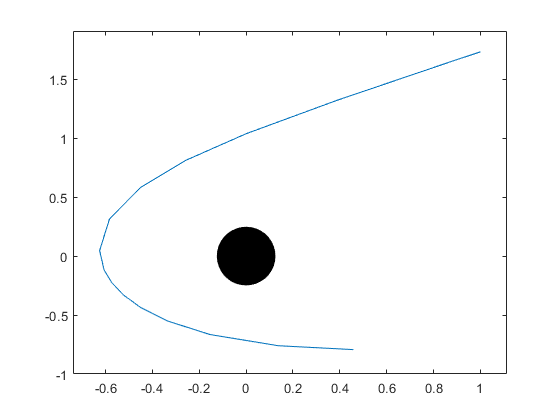
\includegraphics[width=0.495\textwidth]{Report/Images/3_foton_esc.png}}
\subfigure[\label{rfen}movement for $\mu=1$]{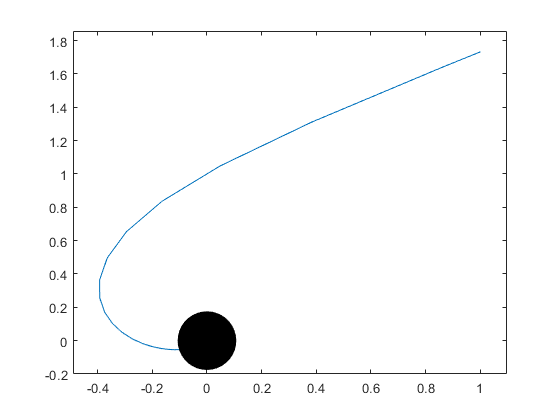
\includegraphics[width=0.495\textwidth]{Report/Images/3_foton_en.png}}
\caption{Solutions of the radial equation}
\end{figure}

\subsubsection{Radial movement $(\dot{\phi}=0)$}
Returning to equation \ref{f2} and conditioning to radial motion, we get that
 \begin{eqnarray*}
       c^{2}\Big( 1- \frac{2\mu}{r}\Big) \dot{t}^{2}-\Big( 1-\frac{2\mu}{r}\Big)^{-1} \dot{r}^{2}&=&0\\
       \pm  c\Big( 1- \frac{2\mu}{r}\Big)&=&\frac{dr}{dt}
\end{eqnarray*}
whose solution is of the form
  \begin{eqnarray}
       ct=\pm r\pm Ln\Big| \frac{r}{2\mu}-1 \Big|+const\label{frf}
 \end{eqnarray}
 For simplicity in this case we will use $cont=0$. from the equation \ref{frf} it can be observed that:
\begin{itemize}
    \item Is valid for outgoing photons $(+)$ an for incoming photons $(-)$.
    \item if $t\rightarrow -t$ then the incoming photons become incoming and the same with incoming.
    \item if $r \rightarrow \infty$ the linear term dominates over the logarithmic, obtaining $ct=r$ that is the form of the standard special-relativistic lightcone. This makes sense since when moving away from the object that curves space-time the geometry of the tends to become flat, more exactly it tends to the geometry of special relativity
    \item if $r \rightarrow 2\mu$ then $ct\rightarrow \infty$ making the light cone completely vertical. The implications of this are better explained with the example of the observer who throws an object in a radial direction (Figure \ref{radm}), while the object is closer to $2\mu$ its cone of light is more vertical, but the cone of light defines the possible future locations of the object then the object would need an infinite time to reach $2\mu$. On the other hand, it also takes an infinite time for the observer to see the object at $2\mu$, since the limits of the light cone also define the movement of the photons emitted by the object.
\end{itemize}

 \begin{figure}[h!]
    \centering
    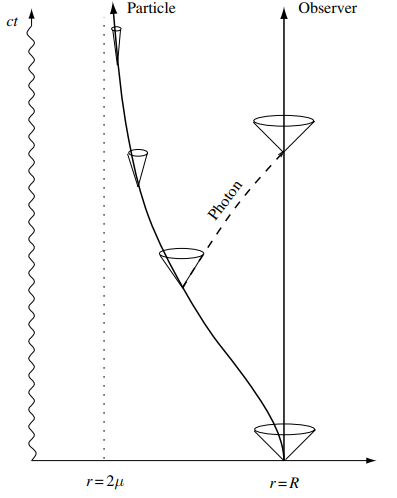
\includegraphics[width=0.5\textwidth]{Report/Images/3_foton_radia.png}
    \caption{{\color{red} ESTAAA}Illustration of the radial movement.}
\label{radm}
\end{figure}

\subsubsection{Circular movement $(\dot{r}=0)$}
Using the radial equation (\ref{fr}) and imposing the condition of radius, verify how easy it is to get to
\begin{eqnarray*}
          R=3\mu=\frac{3GM}{c^{2}}
\end{eqnarray*}
where $R$ is the only radius that allows a circular motion, $R$ being the only radius that allows a circular movement, this radius being too small a quantity so it is not observable for large objects, in the case of our sun we have $R \approx 4.5 Km$. Furthermore, it will later be shown that this orbit is extremely unstable.

\subsubsection{Effective potential and orbits}
Picking up the equation \ref{aste} it is obtained that
\begin{eqnarray}
      \frac{1}{h^{2}}\dot{r}^{2}+\overbrace{\frac{1}{r^{2}}\Big( 1- \frac{2\mu}{r}\Big)}^{V_{eff}}&=& \overbrace{c^{2}k^{2}/h^{2}}^{1/b^{2}} \nonumber\\
      \dot{r}^{2}+V_{eff}&=& \frac{1}{b^{2}} \label{Veff}
\end{eqnarray}
    This effective potential is as shown in Figure \ref{fpot}, having a maximum value of $\frac{1}{ 27\mu^{2}}$ in $3\mu$, said maximum is an unstable equilibrium point and is located in the radius of the circular orbits, therefore these being unstable orbits.\\
 \begin{figure}[h!]
    \centering
    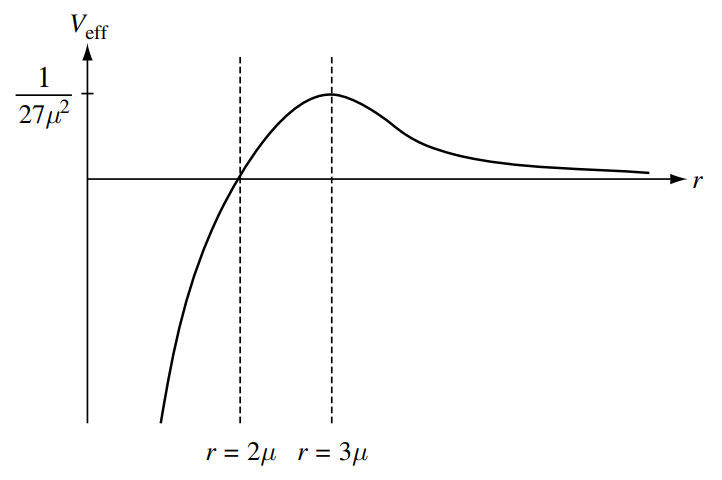
\includegraphics[width=0.65\textwidth]{Report/Images/3_poten.png}
    \caption{Graph of effective potential.}
\label{fpot}
\end{figure}
Then, if we take equation \ref{aste} we can arrive at that
\begin{eqnarray}
\frac{dr}{d\phi}&=&r^{2}\Big(\frac{1}{b^{2}}-V_{eff}\Big)^{1/2}\label{b}
\end{eqnarray}\\
If the equation \ref{b} is observed, it can be deduced that
\begin{itemize}
    \item If $\frac{1}{b^{2}}<\frac{1}{27\mu^{2}}$ $\Rightarrow b>3\sqrt{3}\mu$  then there are going to be values of r in veff that are not allowed, therefore this type of trajectories are the ones that are attracted but do not fall within the massive object.
    \item If $\frac{1}{b^{2}}>\frac{1}{27\mu^{2}}$ $\Rightarrow b<3\sqrt{3}\mu$ are the photons that are attracted and spiral down to the massive object.
\end{itemize}
finally is necessary to physically characterize the constant b, for this we take the equation \ref{b} and see what happens if $r\rightarrow \infty$, arriving at
\begin{eqnarray*}
    \frac{d\phi}{dr}&=&\pm \frac{1}{r^{2}}b\\
    \phi&=&\mp \frac{1}{r}b\\
\end{eqnarray*}
then, if $\phi << 1$ then
\begin{eqnarray*}
       sen(\phi)&=&\mp \frac{1}{r}b \\
       rsen(\phi)=y&=&\mp b\\
\end{eqnarray*}
obtaining that b is the impact parameter of the photon, this is illustrated in the figure \ref{bp}
 \begin{figure}[h!]
    \centering
    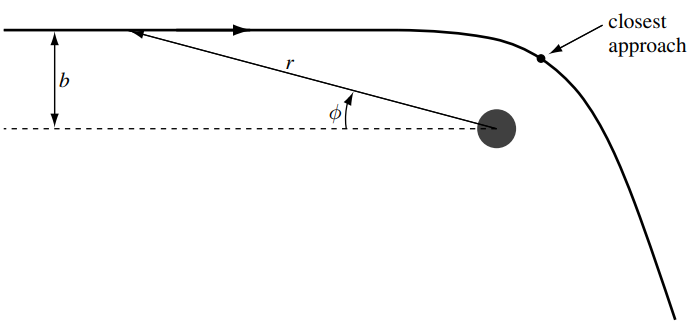
\includegraphics[width=0.65\textwidth]{Report/Images/3_foton_esc_b.png}
    \caption{Illustration of the movement of a photon.}
\label{bp}
\end{figure}
\subsubsection{Redshift in general relativity}
To study the redshift under the Schwarzschild metric, we start by assuming an observer A with a 4-velocity $U_{E}(A)_{\mu}$ that launches a photon with 4-momentum $p_{\mu}$, this photon is seen by another observer B with a 4-speed $U_{R}(B)_{\mu}$ (this experiment mental is best illustrated in figure ref), then its energy can be calculated as:
\begin{eqnarray*}
          E(A)&=&u_{\mu}(A)p_{\mu}(A)\\
          E(B)&=&u_{\mu}(A)p_{\mu}(B)\\
\end{eqnarray*}
then
\begin{eqnarray*}
         \frac{E(A)}{E(B)} &=&\frac{u_{\mu}(A)p_{\mu}(A)}{u_{\mu}(A)p_{\mu}(B)}
\end{eqnarray*}
\begin{figure}[h!]
    \centering
    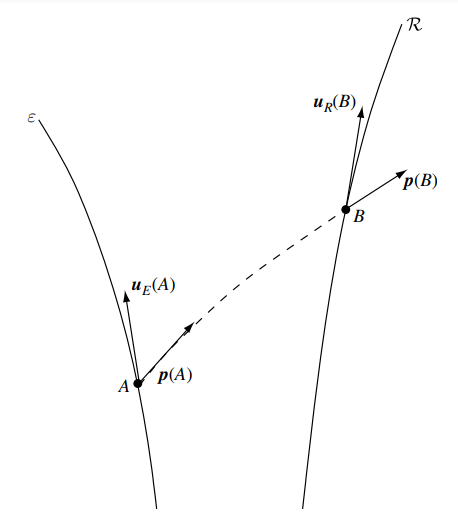
\includegraphics[width=0.6\textwidth]{Report/Images/3_foton_redshift.png}
    \caption{Redshift experiment illustration.}
\label{rs}
\end{figure}
if we consider that both the emitter and the receiver are at rest, it follows that
        \begin{eqnarray*}
    c^{2}&=& g_{\mu nu} u^{\mu}u^{\nu} \\     
            \frac{c}{\sqrt{g_{00}}}&=&u^{0}\\
         \frac{\nu_{A}}{\nu_{B}} &=&\frac{p_{0}(A)}{p_{0}(B)}  \sqrt{\frac{g_{00}(B)}{g_{00}(A)}}
    \end{eqnarray*}
finally knowing that the moment moves in the path as a parallel transport and also having our first integral $p^{\mu}p_{\mu} = 0$, we arrive at that p is constant, obtaining that

        \begin{eqnarray*}
         \frac{\nu_{A}}{\nu_{B}} &=&  \sqrt{\frac{g_{00}(B)}{g_{00}(A)}}
    \end{eqnarray*}

\section{Black Holes}
\subsection{Schwarzschild metric}

This metric i'ts the first exact solution to Einstein field equations for a static, empty spatially isotropic spacetime outside a spherically symmetric body of mass M. In the same way, the Birkhoff's theorem states that the spacetime geometry outside a general spherically symmetric matter distribution is the Schwarzschild geometry.
Based on the previously written, consider a body of mass $M$ and let $\mu = GM/c^2$, then the Schwarzschild metric it's given by the line element:

\begin{block}{}
\begin{equation}
	ds^2 = c^2 \left( 1 - \frac{2\mu}{r}\right) dt^2 - \left( 1 - \frac{2\mu}{r}\right)^{-1} dr^2 - r^2 d\theta^2 - r^2 \sin^2 \theta d\phi^2 \label{2}
\end{equation}
\end{block}
This line element is expressed on the Schwarzschild coordinates $(t,r,\theta,\phi)$ so we use this coordinates to label events in spacetime.\\
I'ts easy to recognize the components of the metric tensor accord to the ussual expression for the line element:
\begin{equation*}
    ds^2 = g_{\mu \nu} x^\mu x^\nu
\end{equation*}
Let $\left( 1 - \frac{2\mu}{r}\right)^{-1}=a$, then: $g_{tt}=c^2a^{-1}$, $g_{rr}=-a$, $g_{\theta \theta}=-r^2$, $g_{\phi \phi}=-r^2sin{^2}\theta$.


\subsection{Regions and singularities on Schwarzschild geometry}
Regions on Schwarzschild geometry are determinated by the hypersurface $r_s=2\mu$ who is known as Schwarzschild radius. Then, the exterior region is $(R_{\mathrm{I}})$: $r>r_s$ and the interior region $(R_{\mathrm{II}})$: $r<r_s$.\\
In general, the Schwarzschild radius lies deep within the body (for example, $r_s$ for the sun is much smaller than his radius). Compact bodies who has a radius similar to $r_s$ are the objects of studio on this section.\\
To establish whether at some event P a
 coordinate $x^\mu$ is timelike, null or spacelike, let see how are the metric components on both regions (those have the information of the tangent vectors to the coordinates, $e^\mu$). For the first region $(R_{\mathrm{I}})$, $g_{tt}>0$ and $(g_{rr}, g_{\theta \theta}, g_{\phi \phi})<0$  thus the coordinate $t$ is timelike and the others are spacelike (t is the proper time measured by an observer at rest at infinity).  For the second region $(R_{\mathrm{II}})$ the metric components $(g_{tt}, g_{rr})$ change sign, therefore the coordinate $t$ is spacetime and $r$ is timelike. Thus, time and radial coordinates changes depending on the side respect of $r_s$.\\
From the line element that describes the Schwarzschild geometry is evident that the metric is singular at $r=0$ and $r=2\mu=r_s$. To see how are the nature of these singularities (coordinate singularity or intrinsec singularity) we consider the physically meaningful geometric quantities that describes the spacetime manifold at any point, the curvature tensor $R_{\mu\nu\rho\sigma}$. Then, spacetime curvature
is described covariantly by the components of this 4-tensor and its contractions. A powerfull tool that its derivated from the curvature tensor is the curvature scalar and its relevance lies in the fact that its value remains the same in all coordinate systems (because its a scalar). From the Schwarzschild metric, the curvature scalar at any point is given by:
\begin{equation*}
    R_{\mu\nu\rho\sigma}R^{\mu\nu\rho\sigma}=\frac{48\mu^2}{r^6}
\end{equation*}
This scalar is singular at $r=0$, then this point is an intrinsic singularity of the Schwarzschild geometry thus is a singularity on spacetime; at this point the curvature of spacetime becomes infinite and the metric (thus the spacetime) isn't well defined. On the other hand, this scalar isn't singular at $r_s$, then this point is a coordinate singularity and the spacetime curvature don't have a singularity on it, thus nothing is occurring in the intrinsic Schwarzschild geometry; this coordinate singularity of the Schwarzschild metric is a result of the coordinate system that we have chosen to use, then we can remove it by making appropriate transformations
of coordinates where the resulting metric will still be a solution of the field equations.

\subsection{Radial photon worldlines in Schwarzschild coordinates}
For a radially moving photon we obtained a solution for the movement equations that is given by:

\begin{equation}
ct=\pm r\pm Ln\Big| \frac{r}{2\mu}-1 \Big|+cte \label{3}\\
\end{equation}

where the minus sign corresponds to a photon that is incoming and the plus sign corresponds to a photon that is outgoing. When we use the transformation $t\rightarrow -t$, the outgoing and incoming photon paths are interchanged, and this is how the $t$ coordinates changes on both regions.\\
The spacetime diagram show the $(r,ct)$-plane for fixed values of $\theta$ and $\Phi$ and on it we plot the paths of radially outgoing and incoming photons, with that the lightcone structure of the Schwarzschild solution its appreciable. The diagram will be the same for all other $\theta$ and $\Phi$ so each point $(r,ct)$ represents a $2$-sphere of area $4\pi r^2$.
\\
\begin{figure}[h!]
    \centering
    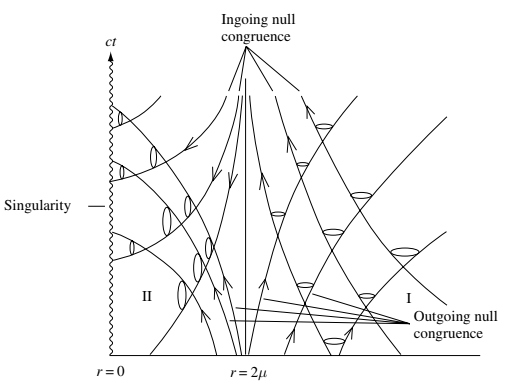
\includegraphics[width=0.58\textwidth]{Report/Images/4bhphotons.png}
    \caption{Ligthcone structure of the Schwarzschild solution on Schwarzschild coordinates.}
\label{fig3}
\end{figure}
In the first region $(R_{\mathrm{I}})$:
\begin{itemize}
\item When $r\rightarrow \infty$ $\Rightarrow$ the term $r$ dominates upon the logarithm then we have $ct=r$ and the metric tends to the Minkowski metric of special relativity. For this large radius the gravitational field becomes weak and the curvature of spacetime isn't appreciable, that's the reason of how the spacetime becomes to be a plane spacetime. The ligthcone structure becomes that of Minkowski spacetime where outgoing and incoming light rays define straight lines of slope $\pm1$ in the diagram.

\item When $r\rightarrow 2\mu$ $\Rightarrow$ The logarithm tends to $\infty$ thus $t\rightarrow \pm\infty$ where the plus sign corresponds to ingoing ligth rays and the minus sign to outgoint light rays. We can conclude that an incoming signal cross the Schwarzschild radius at an infinite time but this isn't visible on figure. On the other hand, the ligthcone it's getting narrower once we aproximmate to the Schwarzschild radius.\\

\end{itemize}
On second region $(R_{\mathrm{II}})$:
\begin{itemize}
  \item  Coordinates $t$ and $r$ reverse their character, then the lightcones flip their orientation by $90^{\circ}$. In this region, all photons must end up at $r=0$ and it follows that this point is a real singularity where the curvature of the Schwarzschild metric diverges (is a point of infinite curvature). Once within the second region  all the photons end up at a intrinsic singularity at $r=0$.
  \item In this region, any massive particle
will end up at the singularity because a timelike worldline must lie inside the forward light-cone at each point.

\end{itemize}
\subsection{Radial particle worldlines in Schwarzschild coordinates}

Consider an infalling particle released from rest at infinity. We can parameterize the particle worldline in terms of the propper time $\tau$, then the trajectory $r(\tau)$ is implicitly given by equation \ref{28}. On the other hand, we can parameterize in terms of the coordinate time $t$, so the trajectory $r(t)$ is implicitly given by equation \ref{29}. With those equations we can plot out the particle trajectory in the $(r,ct)-$plane and the resulting curve is shown in figure (aquí va). \\
From the plot, we can see that the particle worldline has a singularity at $r=2\mu$ and that it takes an infinite coordinate time $t$ for the particle
to cross the Schwarzschild radius. In terms of the proper time, the particle reaches $r_s$ at a finite $\tau$ and for his later values the particle worldline lies in the second region; on this region although $\tau$ continues to increase until $r=0$ is reached,  $t$ decreases along the particle worldline. Although the coordinate $t$ has a physically meaningful as $r\rightarrow \infty$, it's inappropriate for describing particle motion at second region.

\subsection{Eddington-Finkelstein coordinates}

To relabel events in spacetime and remove coordinates singularities, which has resulted simply from choosing coordinates with a restricted domain of validity, we apply some coordinate transformation $x^{\mu}\rightarrow x^{'\mu}$. A possible different set of coordinates is given by the null worldlines of radially moving photons (null geodesics of photons) who is expressed on equation \ref{3}. We take the worldline who corresponds to an ingoing photon and we use the integration constant as the new coordinate, denoted by $p$, then the coordinate transformation is given by 

\begin{equation}
    p= ct + r + Ln\Big| \frac{r}{2\mu}-1 \Big|\label{4}
\end{equation}

We will change the coordinate $t$ for $p$ who is known as the advanced time parameter and is a null coordinate; additionally, $p$ is constant along the entire geodesic of the radially ingoing photon so that make it an optimus coordinate to describe every place where the worldline penetrates.\\
Differentiating \ref{4}: 
\begin{equation*}
    dp= cdt +\frac{r}{r-2\mu}dr=cdt+adr 
\end{equation*}
To obtain the correspondent metric for this coordinates, called ingoing Eddington-Finkelstein coordinates, we obtain an expression for $dt^2$ from the last equation:
\begin{equation*}
    dt= \frac{1}{c} (dp-adr)
\end{equation*}
\begin{equation*}
    dt^2= \frac{1}{c^2} (dp-adr)^2
\end{equation*}
Replacing this element on Schwarzschild metric:
\\
\begin{eqnarray*}
    	ds^2 &=&c^2a^{-1}\frac{1}{c^2} (dp-adr)^2 - a dr^2 - r^2 d\theta^2 - r^2 \sin^2 \theta d\phi^2\\
    	ds^2 &=& a^{-1}(dp^2-2apdpdr+a^2dr^2) - a dr^2 - r^2 d\theta^2 - r^2 \sin^2 \theta d\phi^2\\
    	ds^2 &=& a^{-1}dp^2-2dpdr+adr^2- a dr^2 - r^2 d\theta^2 - r^2 \sin^2 \theta d\phi^2\\ 
    	ds^2 &=& a^{-1}dp^2-2dpdr-  r^2 d\theta^2 - r^2 \sin^2 \theta d\phi^2
\end{eqnarray*}
\\
It follows that:
\begin{equation}
ds^2 =\left( 1 - \frac{2\mu}{r}\right)dp^2-2dpdr- r^2 d\theta^2 - r^2 \sin^2 \theta d\phi^2 \label{5}
\end{equation}
We obtained the line element in terms of the parameter $p$ and is evident that the line elemenet is now regular at $r_s$. Thus, the metric is regular for the whole range $0<r<\infty$ which is the coordinate range for an infalling photon geodesic. In this order of ideas, we have two solutions for Einstein field equations on different coordinates where the given by the equation \ref{2}  is valid on the range of coordinates range $2\mu<r<\infty$ and the metric given by the equation \ref{5} is valid for the whole range $0<r<\infty$.
\\We can obtain the paths of null geodesics from \ref{5} taken $ds=d\theta=d\Phi=0$, thus:
\begin{eqnarray*}
\left( 1 - \frac{2\mu}{r}\right)dp^2-2dpdr&=&0\\
\left( 1 - \frac{2\mu}{r}\right)\frac{dp^2}{dr^2}-2\frac{dp}{dr}&=&0\\
\frac{dp}{dr}\left[\left( 1 - \frac{2\mu}{r}\right)\frac{dp}{dr}-2\right]&=&0
\end{eqnarray*}
This equation has two solutions:

\begin{eqnarray*}
\frac{dp}{dr}&=&0  \ \ \ \ \ \ \ \  \ \ \ \ \ \ \ \ \ \ \ \ \ \ \ \Rightarrow \ \ \ \  p=cte \\
\frac{dp}{dr}&=&2\left( 1 - \frac{2\mu}{r}\right)^{-1}
 \ \ \ \ \ \Rightarrow \ \ \ \ \ p=2r+4\mu Ln\Big| \frac{r}{2\mu}-1 \Big|+cte 
\end{eqnarray*} 

The first solution corresponds to incoming radial null geodesics and the second one to outgoing radial null geodesics. These solutions are valid and congruents with the coordinates construction.\\

We can get a timelike coordinate $t'$ from the null coordinate $p$ and make a new coordinates system wich is called advanced Eddington-Finkelstein coordinates $(t',r,\theta,\phi)$. These coordinate $t'$ is given by:

\begin{equation}
    ct'= p-r=ct+2\mu Ln\Big| \frac{r}{2\mu}-1 \Big|
\end{equation}
Differentiating: 
\begin{equation*}
    dt'= dt +\frac{2\mu}{c}\frac{1}{r-2\mu}dr=dt+\frac{2\mu}{c}\frac{a}{r}dr 
\end{equation*}
To obtain the correspondent metric for this coordinates we obtain an expression for $dt^2$ from the last equation:
\begin{eqnarray*}
    dt&=& dt' -\frac{2\mu}{c}\frac{a}{r}dr \\
    dt^{2}&=& \left(dt' -\frac{2\mu}{c}\frac{a}{r}dr\right)^2
\end{eqnarray*}

Replacing this element on Schwarzschild metric:

\begin{eqnarray*}
    	ds^2 &=&c^2a^{-1}\left(dt' -\frac{2\mu}{c}\frac{a}{r}dr\right)^2 - a dr^2 - r^2 d\theta^2 - r^2 \sin^2 \theta d\phi^2\\
    	ds^2 &=& c^2a^{-1}\left(dt'^2 -\frac{4\mu a}{cr}dt'dr+\left(\frac{2\mu a}{cr}\right)^2dr^2\right) - a dr^2 - r^2 d\theta^2 - r^2 \sin^2 \theta d\phi^2\\
    	ds^2 &=& c^2a^{-1}dt'^2- \frac{4\mu c}{r}dt'dr+\left((2\mu)^2\frac{a}{r^2}-a \right)dr^2- r^2 d\theta^2 - r^2 \sin^2 \theta d\phi^2
\end{eqnarray*}

Making some algebra on the third term of the last equation, we obtain the line element:

\begin{equation}
    	ds^2 &=& c^2\left( 1 - \frac{2\mu}{r}\right)dt'^2- \frac{4\mu c}{r}dt'dr-\left( 1 + \frac{2\mu}{r}\right)dr^2- r^2 d\theta^2 - r^2 \sin^2 \theta d\phi^2
\end{equation}

The line element on advanced Eddington-Finkelstein coordinates $(t',r,\theta,\phi)$ is regular for the whole range $0<r<\infty$ and under the tranformation 
$t'\rightarrow -t'$ the second term changes sign (the line element isn't invariant under the transformation). The regularity implicates that both regions are connected, so we have removed the coordinate singularity. Incoming and outgoing photon worldlines on this coordinates can be deduced by equation \ref{6} and the obtained for the paths of null geodesics given by $p$ for outgoing and incoming photons. 
\begin{eqnarray*}
    	ct'&=&p-r=cte-r\\
    	ct'&=&p-r=r+4\mu Ln\Big| \frac{r}{2\mu}-1 \Big|+cte 
\end{eqnarray*}
The first equation corresponds to ingoing photons and the second one for outgoing photons. Let see the spacetime diagram of the Schwarzschild geometry in advanced Eddington–Finkelstein coordinates with figure \ref{fig11}.
\begin{figure}[h!]
    \centering
    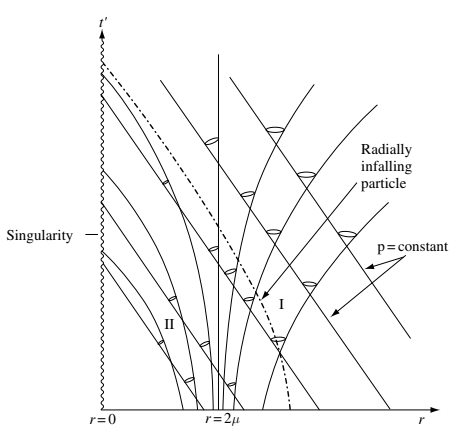
\includegraphics[width=0.57\textwidth]{Report/Images/4bhfinkelstein.png}
    \caption{Ligthcone structure of the Schwarzschild solution on advanced Eddington-Finkelstein coordinates.} 
\label{fig11}
\end{figure}\\
The equation for incoming photons corresponds to a straight line who makes an angle of $45^\circ$with the $r-$axis and is valid for the whole range $0<r<\infty$. On this way, the photon geodesics are continuous straight lines across $r_s$. On these coordinates, the radial trajectory of an infalling particle or photon is continuous but the outgoing null rays are discontinuous at the Schwarzschild radius. The lightcone structure changes at the boundary of Schwarzschild radius, there the future is directed towards the singularity thus once a particle crosses this radius it must fall to the singularity. Another evident phenom is that any particle (massless or not) who starts at second region cannot escape to the  first region, on this sense, the Schwarzschild radius defines an event horizon, a boundary of no return. We can conclude by this definition that a compact object that has an event horizon is called a black hole.\\

We can obtain a new coordinate system based on the worldlines of radially outgoing photons. Analogously to the last construction, we introduce a new null coordinate $q$, wich is known as the retarded time parameter, defined by:
\begin{equation}
    q= ct - r - Ln\Big| \frac{r}{2\mu}-1 \Big|\label{46}
\end{equation}
Following a procedure similar to that used for $p$ we obtain the line element in terms of $q$, wich is regular for the whole range $0<r<\infty$ :
\begin{equation}
ds^2 =\left( 1 - \frac{2\mu}{r}\right)dq^2+2dqdr- r^2 d\theta^2 - r^2 \sin^2 \theta d\phi^2 \label{5}
\end{equation}
Similarly, we obtain a timelike coordinate $t^{''}$ defined by
\begin{equation}
    ct''= q+r=ct-2\mu Ln\Big| \frac{r}{2\mu}-1 \Big|\label{6}
\end{equation}
The coordinates $(t'',r,\theta,\phi)$ are called retarded Eddington–Finkelstein coordinates. On this coordinates appears a mathametical object who is called a white hole and corresponds to the second region (where we found a white hole singularity) and the ingoing null rays are discontinuous. Since the original coordinates covered only a part of the full Schwarzschild geometry, it's necessary introduce new coordinates to extend the solution. Thus, the advanced Eddington–Finkelstein coordinates extend the solution into the part of the manifold that constitutes a black hole, whereas the retarded Eddington–Finkelstein coordinates extend the solution into a different part of the manifold, corresponding to a white hole. 

\subsection{Kruskal coordinates}
Since the Eddington–Finkelstein coordinates don't covered the entire geometry, we are able to introduce a coordinates system who can cover the full Schwarzschild geometry. On this way, we take the difference between the advanced coordinate $p$ and the retarded coordinate $q$ as a transformation for the coordinate $r$, it follows that:
%On these coordinates,the incoming and outgoing radial photons geodesics are continuous straight lines
\begin{equation*}
    \frac{1}{2}(p-q)=r+2\mu Ln\Big| \frac{r}{2\mu}-1 \Big|
\end{equation*}
Taking the sum between $p$ and $q$, we have the transformation for the coordinate $t$, thus:
\begin{equation*}
    \frac{1}{2}(p+q)=ct
\end{equation*}
To obtain the correspondent metric for this coordinates we obtain an expression for $cdt^2$ and for $dr^2$ from the last equations:
\begin{eqnarray*}
dr&=& \frac{1}{2}a^{-1}(dp-dq)\\
dr^2&=& \frac{1}{4}a^{-2}(dp-dq)^2\\
    cdt&=& \frac{1}{2}(dp+dq) \\
    c^{2}dt^{2}&=& \frac{1}{4}(dp+dq)^2
\end{eqnarray*}

Replacing those elements on Schwarzschild metric:
\begin{eqnarray*}
    	ds^2 &=&c^2a^{-1}\frac{1}{c^2} (dp-adr)^2 - a dr^2 - r^2 d\theta^2 - r^2 \sin^2 \theta d\phi^2\\
    	ds^2 &=& a^{-1}(dp^2-2apdpdr+a^2dr^2) - a dr^2 - r^2 d\theta^2 - r^2 \sin^2 \theta d\phi^2\\
    	ds^2 &=& a^{-1}dp^2-2dpdr+adr^2- a dr^2 - r^2 d\theta^2 - r^2 \sin^2 \theta d\phi^2\\ 
    	ds^2 &=& a^{-1}dp^2-2dpdr-  r^2 d\theta^2 - r^2 \sin^2 \theta d\phi^2
\end{eqnarray*}






\subsection{Gravitational collapse and black-hole formation}

\subsection{Tidal forces near a black hole}

\subsection{Hawking effect}

\printbibliography


\end{document}